% ----------------------------------------------------------------------------------------------------- %
% Relatório 1 de PDS - Baseado na classe UFTeX
% ----------------------------------------------------------------------------------------------------- %

\documentclass[tcc]{classe_uftex/uftex}
% ---- Esse comando cria o nome uftex estilizado
\newcommand\uftex{UF\TeX}

\usepackage{lipsum}
\usepackage{tikz}
\usepackage[siunitx]{circuitikz}
\usetikzlibrary{arrows}

\usepackage[alf,abnt-emphasize=bf]{referencias_abnt/abntex2cite}
\renewcommand{\backrefpagesname}{}
\renewcommand{\backref}{}
\renewcommand*{\backrefalt}[4]{}

% ---- Configuração de cores para o código Octave/Matlab
\usepackage{xcolor}
\definecolor{codegreen}{rgb}{0,0.6,0}
\definecolor{codegray}{rgb}{0.5,0.5,0.5}
\definecolor{codepurple}{rgb}{0.58,0,0.82}
\definecolor{backcolour}{rgb}{0.95,0.95,0.92}

\lstset{
    backgroundcolor=\color{backcolour},   
    commentstyle=\color{codegreen},
    keywordstyle=\color{magenta},
    numberstyle=\tiny\color{codegray},
    stringstyle=\color{codepurple},
    basicstyle=\ttfamily\small,
    breakatwhitespace=false,         
    breaklines=true,                 
    captionpos=b,                    
    keepspaces=true,                 
    numbers=left,                    
    numbersep=5pt,                  
    showspaces=false,                
    showstringspaces=false,
    showtabs=false,                  
    tabsize=2
}

% ---- Ajuste para transformar a capa de TCC em Relatório
\makeatletter
\renewcommand\frontpage@maintext{
  \sloppy\nohyphens{Relatório de Laboratório apresentado à disciplina de Processamento Digital de Sinais do curso de \local@deptname\ da \local@universityname .

 \vspace{.5cm}
  \nohyphens{%
    \count1=0
    \@whilenum \count1<\@advisor \do{%
    \ifcase\count1 % same as \ifnum0=\count1
        Professor: \csname uftAdvisorDegree:\the\count1 \endcsname \ 
        \csname uftAdvisorName:\the\count1 \endcsname \ 
        \csname uftAdvisorSurname:\the\count1 \endcsname \ \par
    \else
        \local@coadvisorstring: \csname uftAdvisorDegree:\the\count1 \endcsname \ 
        \csname uftAdvisorName:\the\count1 \endcsname \ 
        \csname uftAdvisorSurname:\the\count1 \endcsname \ \par
    \fi
    \advance\count1 by 1}
  } \par
}
}
\makeatother

% ---- Início do documento
\begin{document}
  % ---- Descrição do título do trabalho 
  \title{Relatório 1 de PDS: Sinais Fundamentais Discretos}
  % ---- Nome do autor ou autores do trabalho
  \author{Maurício}{Moura de Carvalho}
  % ---- Nome do orientador do trabalho.
  \advisor{Prof.}{Ivan}{Ney Alvizuri Romani}{Dr.}

  % ---- Departamento
  \department{EE} % ou o departamento correto
  
  % ---- Data
  \date{17}{03}{2026}
  
  % ---- Palavras-chaves
  \keyword{Processamento Digital de Sinais}
  \keyword{Sinais Discretos}
  \keyword{Octave}

  % ---- Palavras-chaves em inglês
  \foreignkeyword{Digital Signal Processing}
  \foreignkeyword{Discrete Signals}
  \foreignkeyword{Octave}
  
  \maketitle
  \frontmatter

  % ---- Cria o sumário
  \tableofcontents 
  
  % --- Marca o inicio dos elementos textuais
  \mainmatter
  \onehalfspacing

% ----------------------------------------------------------------------------------------------------- %
% Capítulos do trabalho
% ----------------------------------------------------------------------------------------------------- %

\chapter{Introdução}
Este relatório tem como objetivo apresentar os resultados obtidos no primeiro laboratório da disciplina de Processamento Digital de Sinais (PDS), que aborda o tema de Sinais Fundamentais Discretos.

Nesta prática, explorou-se a geração e plotagem de sinais discretos no tempo, bem como operações matemáticas entre eles, através de rotinas desenvolvidas na ferramenta Octave \cite{octaveman}. As atividades seguiram as diretrizes do roteiro de laboratório \cite{roteiro01} e fundamentaram-se na literatura clássica de processamento de sinais \cite{oppenheim, ingle2017}.

\chapter{Metodologia e Procedimentos Práticos}

De acordo com o roteiro do laboratório, foram realizadas a implementação, a plotagem e a análise dos sinais fundamentais e suas operações no Octave. Os procedimentos foram divididos em quatro partes principais:

\begin{itemize}
    \item \textbf{Parte I:} Geração de sinais fundamentais (impulso, degrau, rampa, senoides e exponenciais).
    \item \textbf{Parte II:} Operações aritméticas e deslocamento temporal de sequências.
    \item \textbf{Parte III:} Representação de sequências complexas via translação de impulsos.
    \item \textbf{Parte IV:} Investigação da periodicidade e análise de frequências discretas.
\end{itemize}

O detalhamento de cada item, juntamente com os códigos-fonte e gráficos resultantes, encontra-se no capítulo seguinte.

\chapter{Resultados e Discussões}

\textit{Para melhorar a organização deste relatório, os códigos desenvolvidos em Octave foram separados por item e estão apresentados a seguir, seguidos imediatamente pelos gráficos gerados por eles.}

\section{Resultados da Parte I}

\subsection*{a) Função Impulso Unitário}
\lstinputlisting[language=Matlab, caption={Código gerador do impulso unitário}]{codigos/parte1_a.m}
\begin{figure}[!htpb]
\centering
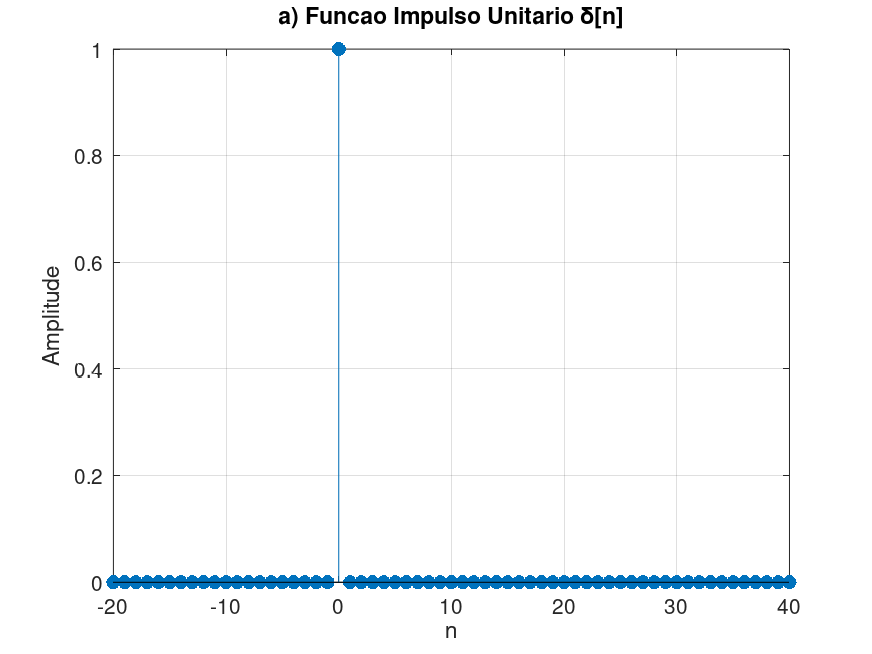
\includegraphics[width=0.8\textwidth]{figuras/parte1_a.png}
\caption{Função Impulso Unitário.}\label{fig:p1a}
\end{figure}

\subsection*{b) Função Degrau Unitário}
\lstinputlisting[language=Matlab, caption={Código gerador do degrau unitário}]{codigos/parte1_b.m}
\begin{figure}[!htpb]
\centering
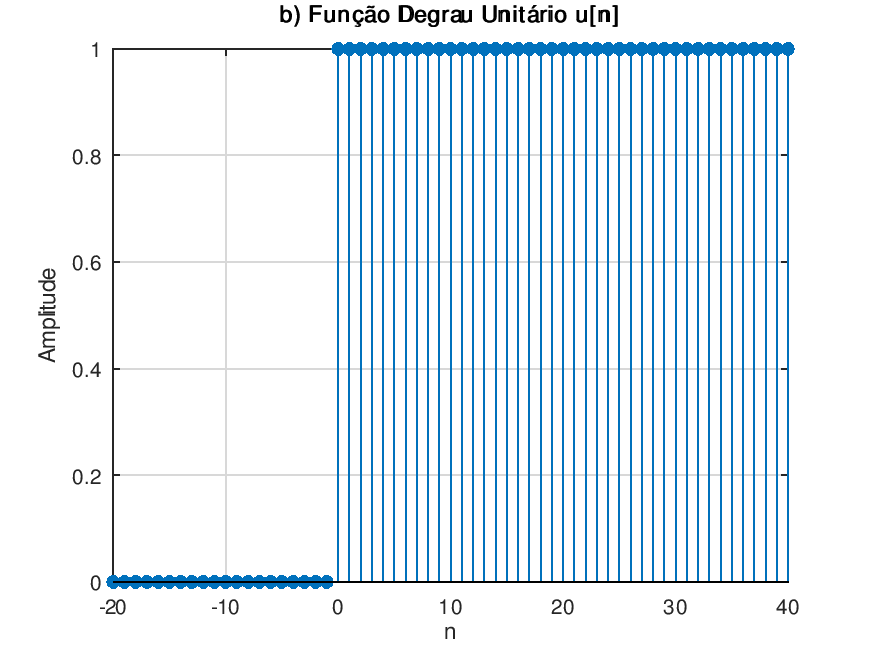
\includegraphics[width=0.8\textwidth]{figuras/parte1_b.png}
\caption{Função Degrau Unitário.}\label{fig:p1b}
\end{figure}

\subsection*{c) Função Rampa}
\lstinputlisting[language=Matlab, caption={Código gerador da rampa}]{codigos/parte1_c.m}
\begin{figure}[!htpb]
\centering
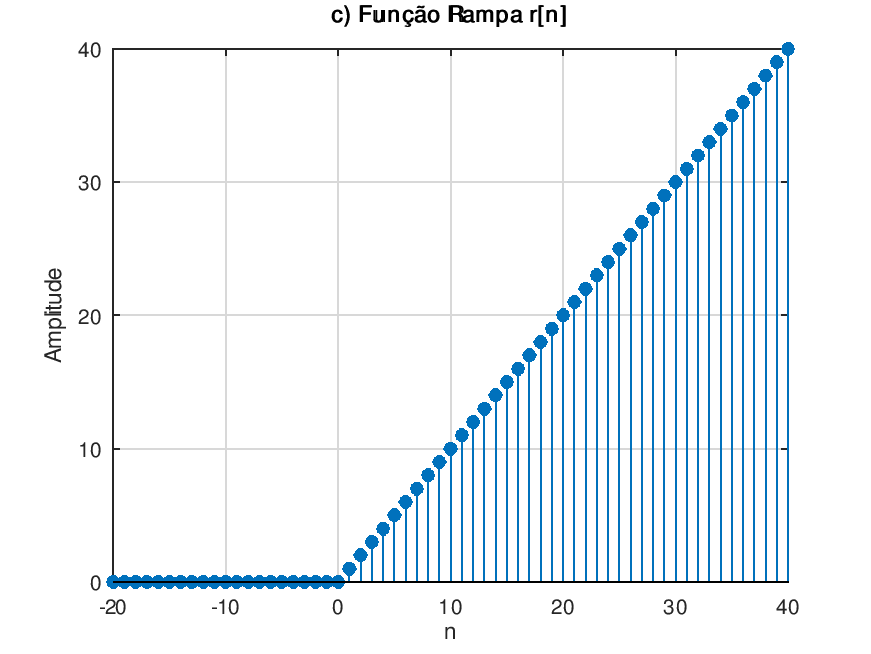
\includegraphics[width=0.8\textwidth]{figuras/parte1_c.png}
\caption{Função Rampa.}\label{fig:p1c}
\end{figure}

\subsection*{d) Sinal Exponencial Real Discreto}
\lstinputlisting[language=Matlab, caption={Código gerador da exponencial real}]{codigos/parte1_d.m}
\begin{figure}[!htpb]
\centering
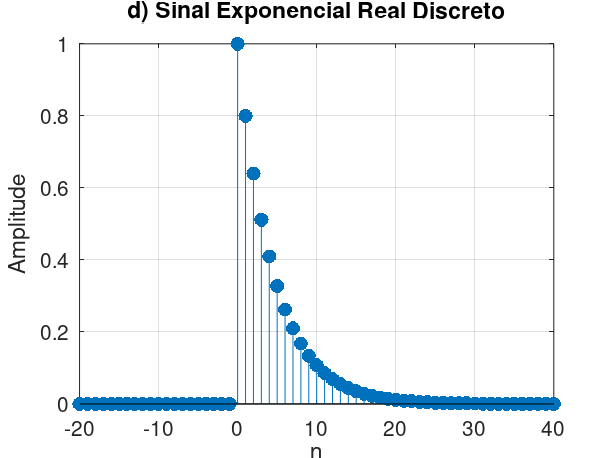
\includegraphics[width=0.8\textwidth]{figuras/parte1_d.png}
\caption{Sinal Exponencial Real.}\label{fig:p1d}
\end{figure}

\subsection*{e) Sinal Senoidal Discreto}
\lstinputlisting[language=Matlab, caption={Código gerador do senoidal}]{codigos/parte1_e.m}
\begin{figure}[!htpb]
\centering
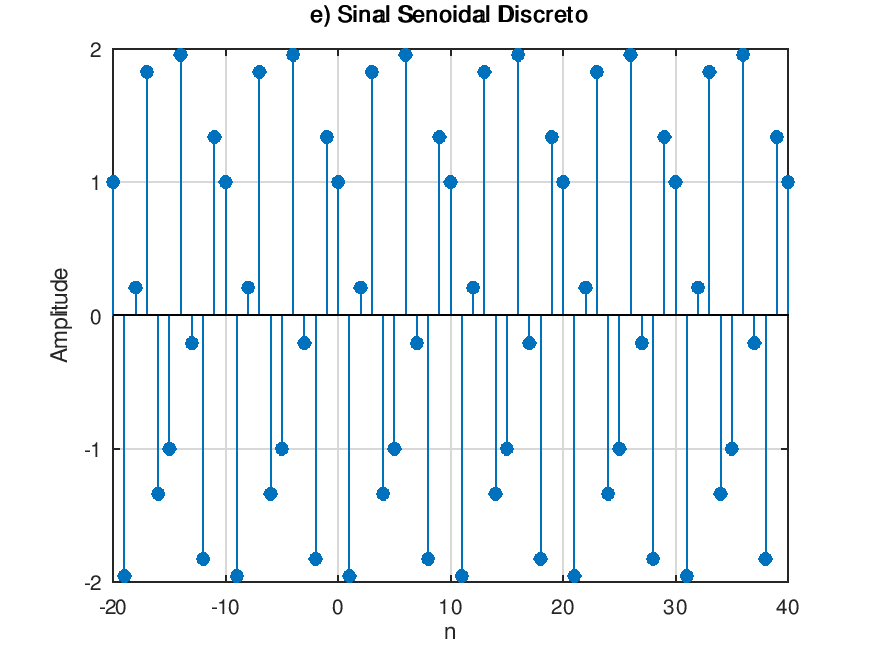
\includegraphics[width=0.8\textwidth]{figuras/parte1_e.png}
\caption{Sinal Senoidal.}\label{fig:p1e}
\end{figure}

\subsection*{f) Sinal Exponencial Complexo}
\lstinputlisting[language=Matlab, caption={Código gerador da exponencial complexa e seus componentes}]{codigos/parte1_f.m}
\begin{figure}[!htpb]
\centering
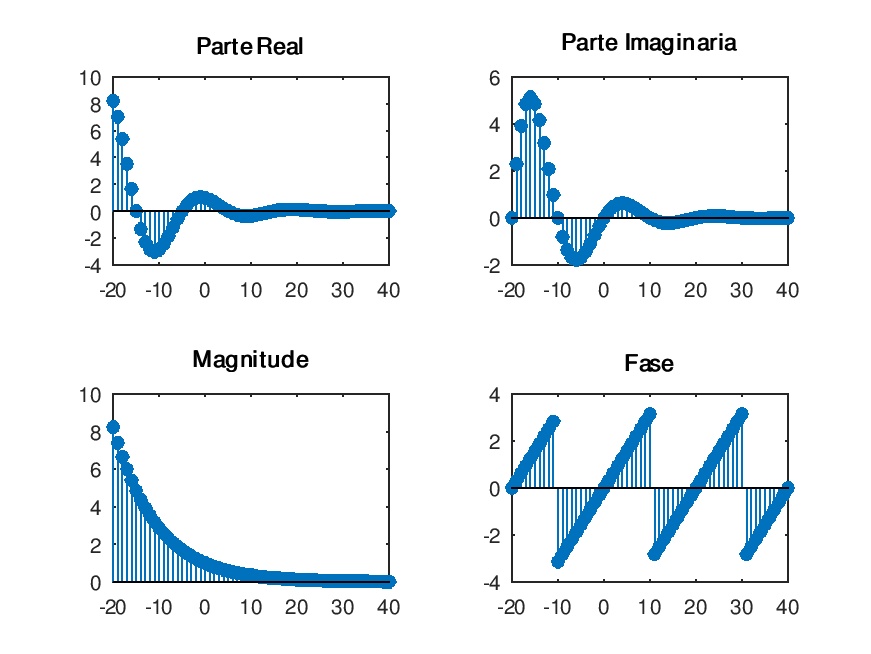
\includegraphics[width=0.8\textwidth]{figuras/parte1_f.png}
\caption{Sinal Exponencial Complexo.}\label{fig:p1f}
\end{figure}

\section{Resultados da Parte II}

\subsection*{a) $X_1[n] = 2A[n] - B[n]$}
\lstinputlisting[language=Matlab, caption={Operação X1}]{codigos/parte2_a.m}
\begin{figure}[!htpb]
\centering
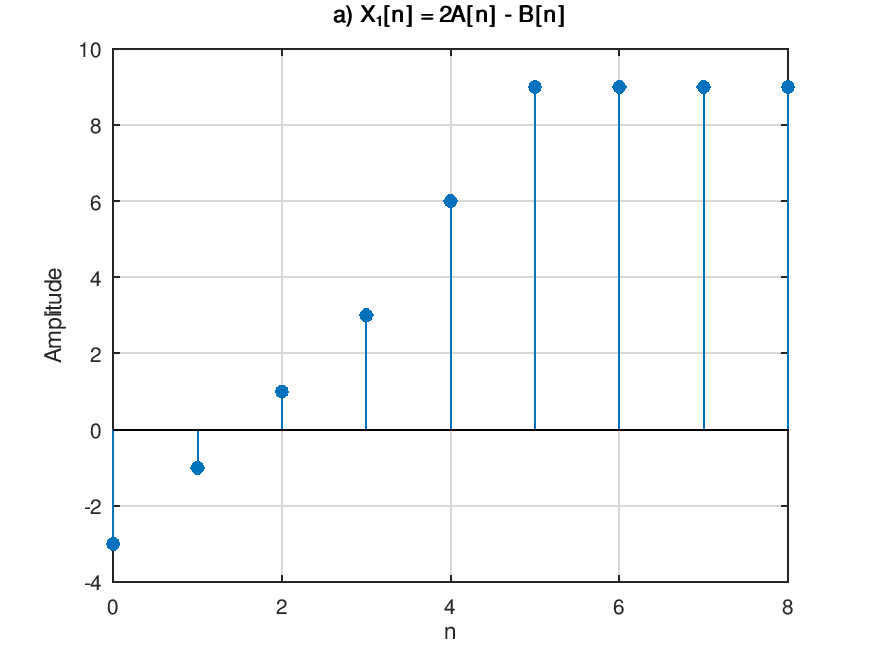
\includegraphics[width=0.8\textwidth]{figuras/parte2_a.png}
\caption{Operação matemática do vetor X1.}\label{fig:p2a}
\end{figure}

\subsection*{b) $X_2[n] = A[n] + 3B[n]$}
\lstinputlisting[language=Matlab, caption={Operação X2}]{codigos/parte2_b.m}
\begin{figure}[!htpb]
\centering
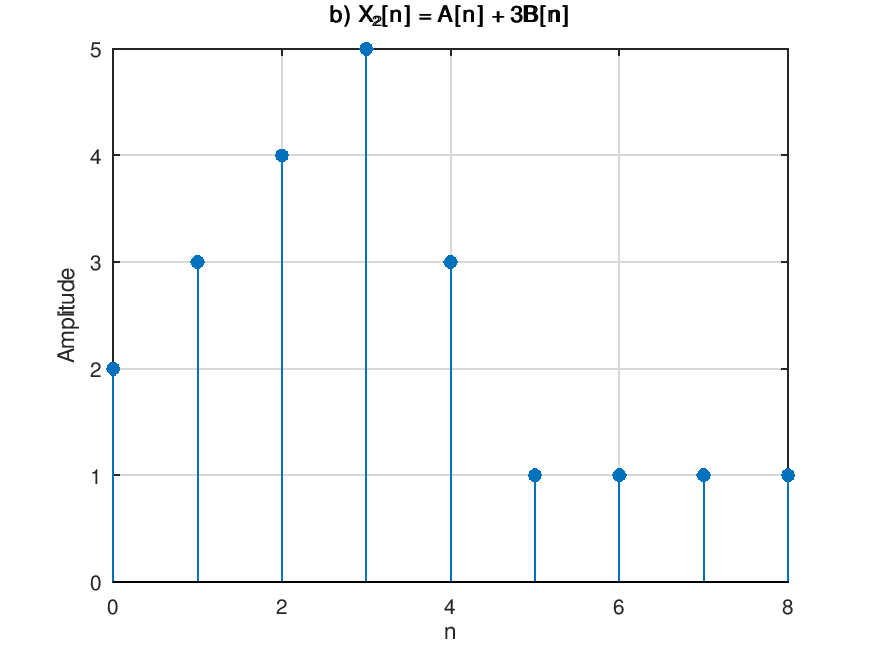
\includegraphics[width=0.8\textwidth]{figuras/parte2_b.png}
\caption{Operação matemática do vetor X2.}\label{fig:p2b}
\end{figure}

\subsection*{c) $X_3[n] = X_2[-n]$}
\lstinputlisting[language=Matlab, caption={Operação X3 com deslocamento}]{codigos/parte2_c.m}
\begin{figure}[!htpb]
\centering
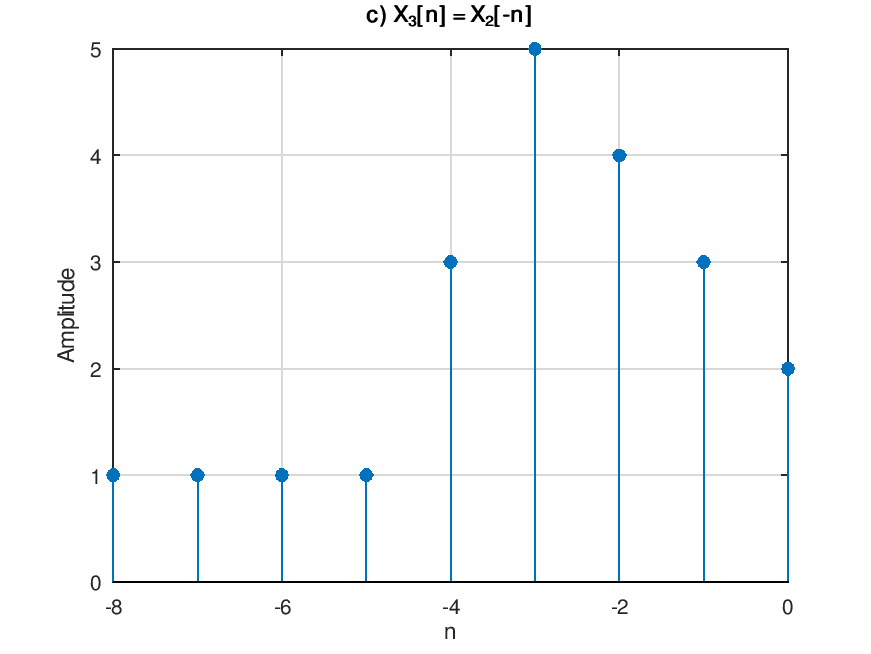
\includegraphics[width=0.8\textwidth]{figuras/parte2_c.png}
\caption{Sinal rebatido no tempo.}\label{fig:p2c}
\end{figure}

\section{Resultados da Parte III}

\subsection*{a) Equação $x[n]$ com impulsos deslocados}
\lstinputlisting[language=Matlab, caption={Código da equação x[n]}]{codigos/parte3_a.m}
\begin{figure}[!htpb]
\centering
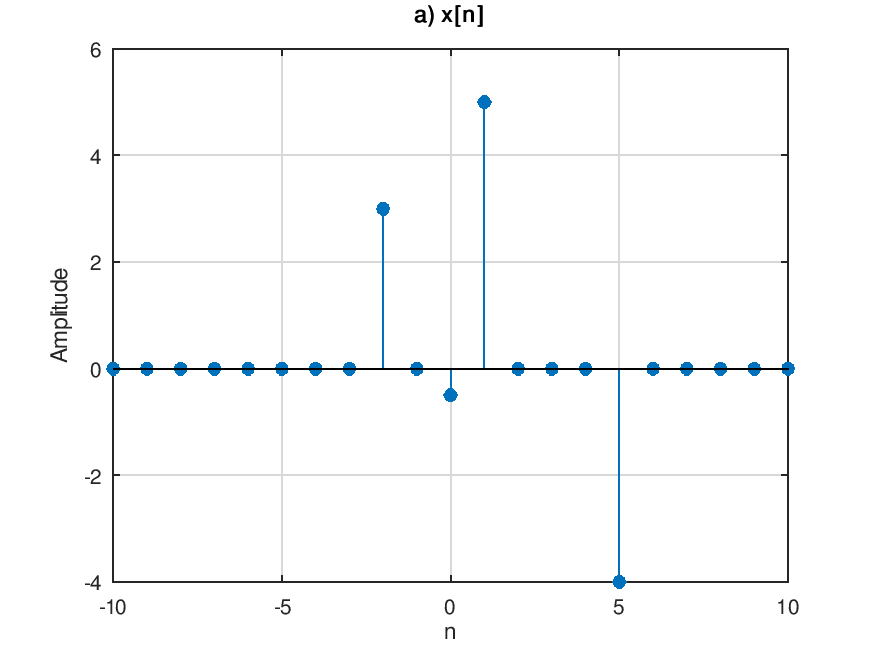
\includegraphics[width=0.8\textwidth]{figuras/parte3_a.png}
\caption{Composição da função x[n] por funções impulso.}\label{fig:p3a}
\end{figure}

\subsection*{b) Equação $y[n]$ com impulsos deslocados}
\lstinputlisting[language=Matlab, caption={Código da equação y[n]}]{codigos/parte3_b.m}
\begin{figure}[!htpb]
\centering
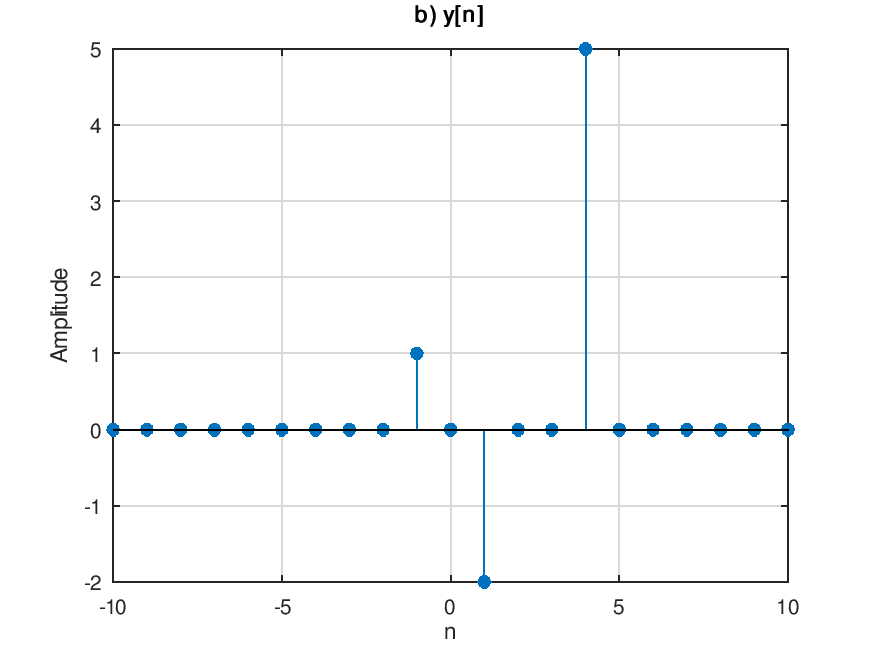
\includegraphics[width=0.8\textwidth]{figuras/parte3_b.png}
\caption{Composição da função y[n] por funções impulso.}\label{fig:p3b}
\end{figure}

\section{Resultados da Parte IV}

\subsection*{a) Sequência $\cos(0,1n - \pi)$ na restrição $[-20, 20]$}
\lstinputlisting[language=Matlab, caption={Código a)}]{codigos/parte4_a.m}
\begin{figure}[!htpb]
\centering
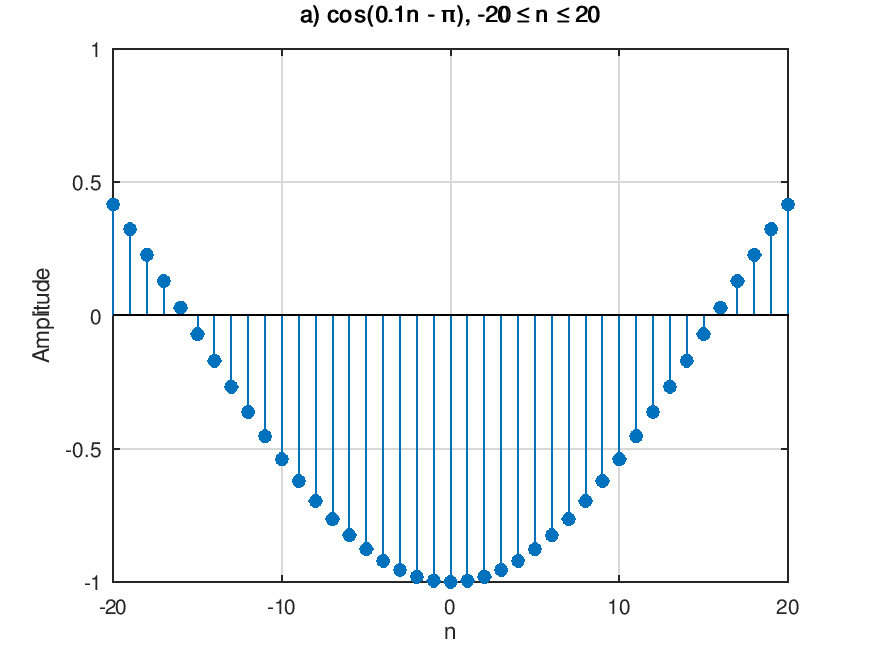
\includegraphics[width=0.8\textwidth]{figuras/parte4_a.png}
\caption{Cossenoide a).}\label{fig:p4a}
\end{figure}

\subsection*{b) Sequência $\cos(0,1n - \pi)$ na restrição $[-10, 20]$}
\lstinputlisting[language=Matlab, caption={Código b)}]{codigos/parte4_b.m}
\begin{figure}[!htpb]
\centering
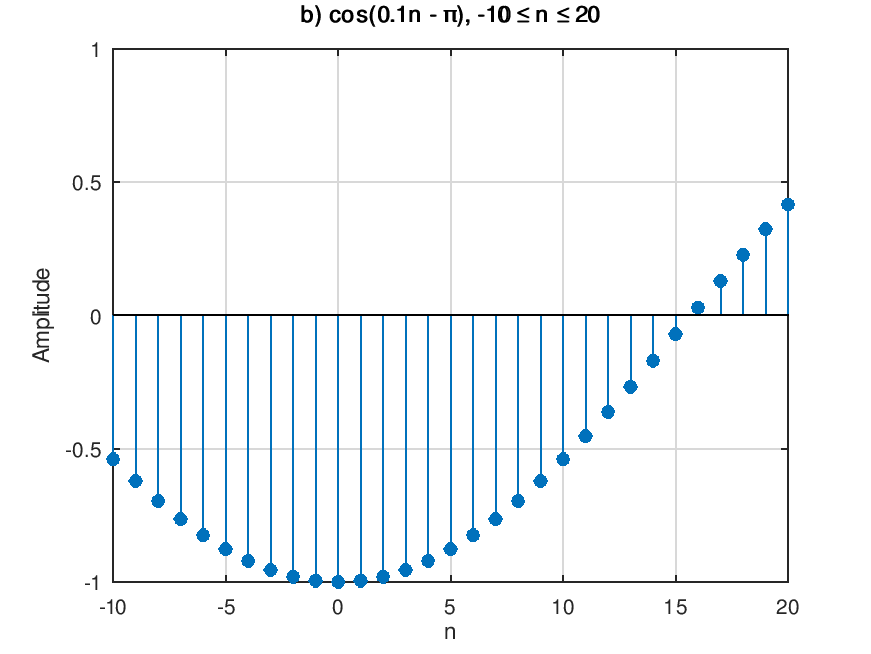
\includegraphics[width=0.8\textwidth]{figuras/parte4_b.png}
\caption{Cossenoide b).}\label{fig:p4b}
\end{figure}

\subsection{Análise de Periodicidade}
Sabe-se que um sinal discreto na forma $\cos(\Omega_0 n + \phi)$ é periódico se, e somente se, a relação $\frac{\Omega_0}{2\pi}$ for um número racional.

No caso proposto, a frequência angular é $\Omega_0 = 0,1$ rad/amostra. Assim, para encontrarmos o período fundamental $N$:
\begin{equation}
    N = \frac{2\pi m}{\Omega_0} = \frac{2\pi m}{0,1} = 20\pi m
\end{equation}

Como não existe um número inteiro $m$ diferente de zero que torne $N$ também um número inteiro (visto que a frequência está atrelada ao número irracional $\pi$), conclui-se que matematicamente \textbf{estas sequências não são periódicas}. No domínio discreto, as amostras não se repetem exatamente nos mesmos valores a cada ciclo.

\chapter{Conclusão}
Este laboratório proporcionou uma compreensão sólida sobre a representação e manipulação de sinais discretos no tempo. A implementação de funções básicas como impulso unitário, degrau, rampa e exponenciais complexas permitiu visualizar as propriedades fundamentais que formam a base do Processamento Digital de Sinais (PDS).

As operações realizadas entre as sequências (soma, multiplicação escalar e rebatimento temporal) demonstraram como manipular digitalmente a informação contida nos sinais. Além disso, a análise de periodicidade reforçou a distinção crítica entre sinais contínuos e discretos, onde a periodicidade não depende apenas da frequência, mas da racionalidade da relação entre a frequência angular e $2\pi$.

A utilização do Octave \cite{octaveman} e a consulta à documentação oficial \cite{matlabdoc} provaram ser ferramentas essenciais para a verificação prática dos conceitos teóricos discutidos em aula e apresentados na literatura \cite{ingle2017}. Conclui-se que o domínio da geração e caracterização destes sinais elementares é um passo indispensável para o estudo de sistemas lineares invariantes no tempo (LIT) e transformadas de frequência que serão abordadas nos próximos módulos da disciplina.

% ----------------------------------------------------------------------------------------------------- %
\backmatter 
\singlespacing   
% ----------------------------------------------------------------------------------------------------- %
\bibliography{relatorio_1}

\end{document}
